\documentclass{article}

\usepackage {amsmath}
\usepackage [margin=2cm]{geometry}
\usepackage {slashed}
\usepackage {graphicx}
\usepackage {subcaption}

\newcommand{\ua}{\uparrow}
\newcommand{\da}{\downarrow}
\newcommand{\mael}{\mathcal{M}}
\newcommand{\gm}{\gamma^{\mu}}

\begin {document}
\section{Di-lepton production in $e^+e^-$ in the SM}

\subsection{Feynman graphs}
\begin{figure}[h!]
  \centering
  \begin{subfigure}[b]{0.4\textwidth}
    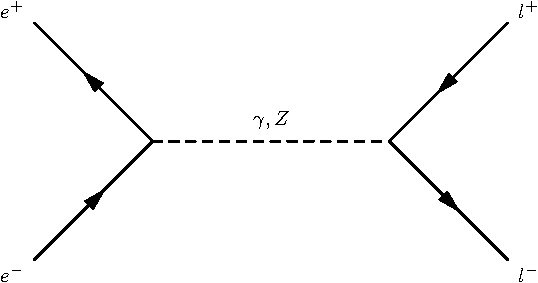
\includegraphics[width=\textwidth]{../graphs/gammaZ.pdf}
  \end{subfigure}
~
  \begin{subfigure}[b]{0.4\textwidth}
    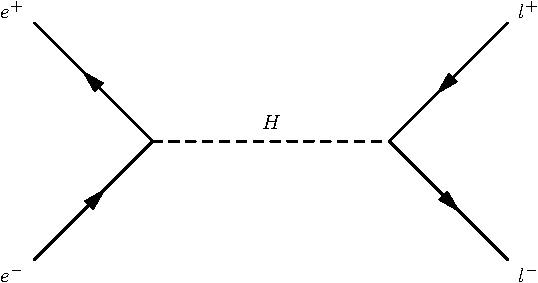
\includegraphics[width=\textwidth]{../graphs/H.pdf}
  \end{subfigure}
\end{figure}
$e^+e^-$ annihiliation into $\gamma$ is the more favourable choice
compared to $Z$ and $H$ due to the mass difference in these.

\subsection{Final states}
The $e$ and $\mu$ are stable particles and will therefore be detected
as particle paths in the calorimeters. $\tau$ has a short life time and
will therefore most likely decay before hitting the detector.
Some decay modes from $\tau$ are
\begin{flalign*}
  \pi^{\pm} + \pi^0 + \nu_{\tau}      &:  &25.52\,\%\\
  e^{\pm} + \nu_{e} + \nu{\tau}	      &:  &17.83\,\%\\
  \mu^{\pm} + \nu_{\mu} + \nu{\tau}   &:  &17.41\,\%\\
  \pi^{\pm} + \nu_{\tau}	      &:  &10.83\,\%\\
  \pi^{\pm} + 2\pi^0 + \nu_{\tau}     &:  &9.30\,\%\\
  K^{\pm} + \nu_{\tau}		      &:  &7.00\,\%
\end{flalign*}


\subsection{QED}
Using the Feynman rules for scalar QED we get an amplitude
%
\begin{equation}
  i\mael =%
		\bar{v}^{s'}(p')(-ie\gm)u^s(p)%
		\left(\frac{-ig_{\mu\nu}}{q^2}\right)%
		\bar{u}^r(k)(-ie\gamma^{\nu})v^{r'}(k')
\end{equation}
%
Where $p$ and $p'$ are the momentum for the incoming $e^+e^-$,%
and $k$ and $k'$ are the momentums of the outgoing $\tau^+\tau^-$.
$s$ and $r$ are the spin indicies, $q$ is the momentum of the force
mediator and $e$ is the elementary charge.
On a more compact form leaving the spin superscripts implicit
%
\begin{equation}
  i\mael =%
		\frac{ie^2}{q^2}\left(\bar{v}(p')\gm u(p)\right)%
		\left(\bar{u}(k)\gamma_{\mu}v(k')\right)
\end{equation}
%
Then using $(\bar{v}\gm u)^* = \bar{u}\gm v$
to get the $|\mael|^2$ leads to
%
\begin{equation}
|\mael|^2 = \frac{e^4}{q^4}%
		  \Big(\bar{v}(p')\gm u(p)\bar{u}(k)\gamma^{\nu}v(k')\Big)%
		  \Big(\bar{u}(k)\gamma_{\mu}v(k')\bar{v}(p')\gamma_{\nu}u(p)\Big)
\label{sqM}
\end{equation}
%
Now taking the spins into account we have an expression on the form
%
\begin{equation}
  \frac{1}{4}\sum_s\sum_{s'}\sum_r\sum_{r'}|\mael(s,s'\rightarrow r,r')|^2.
\end{equation}
%
With the 2 completeness relations
%
\begin{equation}
  \sum_s u^s(p)\bar{u}^s(p) = \slashed{p} + m\,;\quad\quad%
  \sum_s v^s(p)\bar{v}^s(p) = \slashed{p} - m
  \label{comprel}
\end{equation}
%
used in the the first parenthesis in equation (\ref{sqM}) written out in spinor indicies,
making it possible to move $v$ and $\bar{v}$ next to each other we get
\begin{flalign*}
  \sum_{s,s'} \bar{v}^{s'}_{a}(p')\gm_{ab}u^s_b(p)%
  \bar{u}^s_c(p)\gamma^{\nu}_{cd}v^{s'}_d(p') &=%
  (\slashed{p}'-m)_{da}\gm_{ab}(\slashed{p} + m)_{bc}\gamma^{\nu}_{cd}\\
  &= \text{tr}[(\slashed{p}' -m)\gm(\slashed{p}+m)\gamma^{\nu}]
\end{flalign*}
thus our squared matrix element becomes the product of 2 traces
%
\begin{equation}
  \frac{1}{4}\sum_{\text{spins}}|\mael|^2 = %
  \frac{e^4}{4q^4}%
  \text{tr}\left[(\slashed{p}' - m_e)\gm(\slashed{p} + m_e)\gamma^{\nu}\right]%
  \text{tr}\left[(\slashed{k} + m_{\tau})\gamma_{\mu}(\slashed{k}' - m_{\tau})\gamma_{\nu}\right]%
\end{equation}
%
Insert trace technology here
%
Using the trace relations we get for the $e$ part
%
\begin{equation}
  \text{tr}\left[(\slashed{p}' - m_e)\gm(\slashed{p} + m_e)\gamma^{\nu}\right] =%
  4\left[p^{'\mu}p^{\nu} + p^{'\nu}p^{\mu} - g^{\mu\nu}(p\cdot p' + m_e^2)\right]
\end{equation}
and for the $\tau$
\begin{equation}
  \text{tr}\left[(\slashed{k} + m_{\tau})\gamma_{\mu}(\slashed{k}' + m_{\tau})\gamma_{\nu}\right] =%
  4\left[k_{\mu}k'_{\nu} + k_{\nu}k'_{\mu} - g_{\mu\nu}(k\cdot k' + m_{\tau}^2)\right]
\end{equation}
%
There is a large difference in $m_e << m_{\tau}$ which makes it reasonable to set $m_e = 0$,
multiplying the traces gives us a square matrix element of
%
\begin{equation}
  \frac{1}{4}\sum_{\text{spins}}|\mael|^2 =%
  \frac{8e^4}{q^4}%
  \left[(p\cdot k)(p'\cdot k') + (p\cdot k')(p'\cdot k) + m^2_{\tau}(p\cdot p')\right]
  \label{genEq}
\end{equation}
%
Furterhmore we choose the center of mass reference frame and translates our momentums into
kinematic variables instead, energies and angles.
%
\begin{equation}
\begin{array}{ccc}
  q^2 = (p+p')^2 = 4E^2 &\,;\quad& p\cdot p' = 2E^2\\
  p\cdot k = E^2 - E|\textbf{k}|\cos\theta &\,;\quad& p\cdot k' = E^2 + E|\textbf{k}|\cos\theta
\end{array}
\end{equation}
%
Rewriting eq. (\ref{genEq}) in terms of $E$ and $\theta$ we get
%
\begin{flalign}
  \frac{1}{4}\sum_{\text{spins}}|\mael|^2 &=%
  \frac{8e^4}{16E^4}%
  \Big[ %
    E^2(E-|\textbf{k}|\cos\theta)^2 +%
    E^2(E+|\textbf{k}|\cos\theta)^2 +%
    2m_{\tau}^2E^2]
  \Big]\\
  %
  &= e^4%
  \left[ %
    \left(1+\frac{m^2_{\tau}}{E^2}\right) +%
    \left(1 - \frac{m^2_{\tau}}{E^2}\right)\cos^2\theta%
  \right]
\end{flalign}
%
Now that we have $|\mael|^2$  we can put it into a formula for $d\sigma/d\cos\theta$
derived in Peskin\footnote{Page 107, Equation 4.84}
%
\begin{equation}
  \left(\frac{d\sigma}{d\Omega}\right)_{CM} =%
  \frac{1}{2E_A 2E_B |v_p - v_{p'}|}\frac{|\mathbf{k}|}{(2\pi)^24E_{CM}}|\mael|^2
\end{equation}
%
In the center of mass frame the relative speed $|v_{p}- v_{p'}|$ becomes 2, and $E_p=E_{p'}=E_{CM}/2 = \sqrt{s}/2$.
With a symmetry about the longitudinal direction we can make the differential cross section
\begin{equation}
  \frac{d\sigma}{d\cos\theta} = %
  \frac{\mathbf{|k|}}{32\pi^2 s^{3/2}} |\mael|^2 =%
  \frac{1}{32\pi^2s}\sqrt{1-4\frac{m_{\tau}^2}{s}}|\mael|^2
\end{equation}
%
Integrating with respect to $\cos\theta$ we aquire the total cross section. Keeping the prefactors
out of the calculation since they are not dependent on $cos\theta$ and integrate our expression
for the squared matrix element.
%
\begin{flalign*}
  \int^1_{-1}d\cos\theta e^4|\mael|^2 &=%
  e^4\left[\left(1+4\frac{m_{\tau}^2}{s}\right)\cos\theta+%
  \frac{1}{3}\left(1-4\frac{m_{\tau}^2}{s}\right)\cos^3\theta\right]^{1}_{-1}\\
  &= \frac{8}{3}\left(1 + 2\frac{m^2_{\tau}}{s}\right)
\end{flalign*}
Combining combining this with our differential cross section we get an expression for the
total cross section
\begin{flalign*}
  \sigma &=  \frac{4}{3}\frac{e^4}{32\pi^2s}%
  \sqrt{1-4\frac{m^2_{\tau}}{s}}\left(1+2\frac{m^2_{\tau}}{s}\right)\\
  &= \frac{2}{3}\frac{\alpha^2}{s}%
  \sqrt{1-4\frac{m^2_{\tau}}{s}}\left(1+2\frac{m^2_{\tau}}{s}\right)
\end{flalign*}
with $\alpha = e^2/(4\pi)$.


\subsection{Rate}
The distribution of number of events goes as $N = L\times \sigma$, where $L$ is the luminosity
and $\sigma$ is the cross section.

\subsection{$e^+e^- \rightarrow e^+e^-,\mu^+\mu^-,\tau^+\tau^-$}
%
The $e^+e^- \rightarrow e^+e^-$ case we have to extra diagrams where a
photon or a $Z$ are exchanged between $e^+e^-$ without anything changing the outcome,
and would so give this process a higher probability of happening then the others.
The $\tau$ has a much larger mass and would therefore require larger incoming energies
to have enough momenta in the photon to decay to $\tau$.

\subsection{Electroweak}
This unifcation requires both the $\mael_{QED}$ and $\mael_{WI}$
matrix elements. Using the feynman-rules from the weak model our $\mael_{WI}$
will take the form
%
\begin{equation}
  \mael_{WI} = -\frac{g^2_Z}{s - m^2_Z + im_z\Gamma_Z}g_{\mu\nu}%
  \left[\bar{v}(p')\gm\frac{1}{2}(c^e_V - c^e_A\gamma^5)u(p)\right]%
  \left[\bar{u}(k)\gm\frac{1}{2}(c^{\tau}_V - c^{\tau}_A\gamma^5)v(k')\right]
\end{equation}
%
where $1/(s - m^2_Z + im_Z\Gamma_Z) = P_Z(s)$ is the Z propogator, $c^{e/\tau}_{V/A}$
are the vector and axial-vector couplings of the Z to our leptons.
It will be handy to rewrite those couplings to left- and right-handed
chiral states as $c_V = c_L + c_R$ and $c_A = c_L - c_R$
%
\begin{equation}
  -P_Zg_Z^2g_{\mu\nu}%
  \left[%
    c_L^e \bar{v}(p') \gm P_L u(p) +%
    c_R^e \bar{v}(p') \gm P_R u(p) %
  \right]%
  \left[%
    c_L^{\tau} \bar{u}(k) \gamma^{\nu} P_L v(k') +%
    c_R^{\tau} \bar{u}(k) \gamma^{\nu} P_R v(k') %
  \right]
\end{equation}
%
where $P_L$ and $P_R$ are the chiral projection operators $\frac{1}{2}(1\mp \gamma^5)$.
Using these chiral projection operators on a particle state give the result
\[ P_Lu=u_{\da},\, P_Ru = u_{\ua},\, P_Lv = v_{\ua},\, P_Rv=v_{\da} \]
And with helicity combinations like $\bar{u}_{\ua}\gm v_{\ua}$ giving zero
matrix elements we are left with four helicity combinations
%
\begin{flalign}
  \mael_{RR} &=-P_Z g^2_Z c^{e}_{R}c^{\tau}_{R} g^{\mu\nu}%
  \left[ \bar{v}_{\da}(p')\gm u_{\ua}(p)\right]%
  \left[ \bar{u}_{\ua}(k)\gamma^{\nu}v_{\da}(k')\right]\\
  \mael_{RL} &=-P_Z g^2_Z c^{e}_{R}c^{\tau}_{L} g^{\mu\nu}%
  \left[ \bar{v}_{\da}(p')\gm u_{\ua}(p)\right]%
  \left[ \bar{u}_{\da}(k)\gamma^{\nu}v_{\ua}(k')\right]\\
  \mael_{LR} &=-P_Z g^2_Z c^{e}_{L}c^{\tau}_{R} g^{\mu\nu}%
  \left[ \bar{v}_{\ua}(p')\gm u_{\da}(p)\right]%
  \left[ \bar{u}_{\ua}(k)\gamma^{\nu}v_{\da}(k')\right]\\
  \mael_{LL} &=-P_Z g^2_Z c^{e}_{L}c^{\tau}_{L} g^{\mu\nu}%
  \left[ \bar{v}_{\ua}(p')\gm u_{\da}(p)\right]%
  \left[ \bar{u}_{\ua}(k)\gamma^{\nu}v_{\ua}(k')\right]
\end{flalign}
%
The combinations of these four-vector currents can be shown to come to a simpler form
as with this example which is the same as in $QED$
%
\[
  g_{\mu\nu} [\bar{v}_{\da}(p')\gm u_{\ua}(p)]%
  [\bar{u}_{\ua}(k)\gamma^{\nu}v_{\da}(k')] = s(1+\cos\theta)
\]
%
using this on each helicity state we get
%
\begin{flalign}
  |\mael_{RR}|^2 &=|P_Z|^2 g^4_Z (c^{e}_{R})^2(c^{\tau}_{R})^2 (1+\cos\theta)^2\\
  |\mael_{RL}|^2 &=|P_Z|^2 g^4_Z (c^{e}_{R})^2(c^{\tau}_{L})^2 (1-\cos\theta)^2\\
  |\mael_{LR}|^2 &=|P_Z|^2 g^4_Z (c^{e}_{L})^2(c^{\tau}_{R})^2 (1-\cos\theta)^2\\
  |\mael_{LL}|^2 &=|P_Z|^2 g^4_Z (c^{e}_{L})^2(c^{\tau}_{L})^2 (1+\cos\theta)^2
\end{flalign}
%
The spin average of the full matrix elemnt $|\mael|^2$ is then the sum of each helicity
state squared
%
\[
  <|\mael|^2> = \frac{1}{4} \left( |\mael_{RR}|^2 + |\mael_{LL}|^2 +%
  |\mael_{RL}|^2 + |\mael_{LR}|^2\right)
\]
%
writing the terms out gives us
%
\begin{flalign*}
  <|\mael|^2> = %
  \frac{1}{4}|P_Z|^2 g_Z^4 s^2%
  \Big(%
  &\left[ (c^e_R)^2(c^{\tau}_R)^2 + (c^e_L)^2(c^{\tau}_L)^2 \right](1+\cos\theta)^2 \\+%
  &\left[ (c^e_R)^2(c^{\tau}_L)^2 + (c^e_L)^2(c^{\tau}_R)^2 \right](1-\cos\theta)^2%
  \Big)
\end{flalign*}
This is the $|\mael_{WI}|^2$. Now we have to find the cross terms
$\mael^*_{QED}\mael_{WI}$ and $\mael^*_{WI}\mael_{QED}$.
For the first combination we have to combine the $QED$ part with each of the 
helicity combinations of the $WI$
\begin{flalign*}
  &\mael^*_{QED}\mael_{RR} = |P_Z|^2g_Z^4 e^2c^e_Rc^{\tau}_R%
  [\bar{v}_{\da}(k')\gm u_{\ua}(k)][\bar{u}_{\ua}(p)\gamma_{\mu} v_{\da}(p')]%
  [\bar{v}_{\da}(p')\gamma^{\nu} u_{\ua}(p)][\bar{u}_{\ua}(k)\gamma_{\nu} v_{\da}(k')]\\
  %
  &\mael^*_{QED}\mael_{RL} = |P_Z|^2g_Z^4 e^2c^e_Rc^{\tau}_L%
  [\bar{v}_{\ua}(k')\gm u_{\da}(k)][\bar{u}_{\ua}(p)\gamma_{\mu} v_{\da}(p')]%
  [\bar{v}_{\da}(p')\gamma^{\nu} u_{\ua}(p)][\bar{u}_{\da}(k)\gamma_{\nu} v_{\ua}(k')]\\
  %
  &\mael^*_{QED}\mael_{LR} = |P_Z|^2g_Z^4 e^2c^e_Lc^{\tau}_R%
  [\bar{v}_{\da}(k')\gm u_{\ua}(k)][\bar{u}_{\da}(p)\gamma_{\mu} v_{\ua}(p')]%
  [\bar{v}_{\ua}(p')\gamma^{\nu} u_{\da}(p)][\bar{u}_{\ua}(k)\gamma_{\nu} v_{\da}(k')]\\
  %
  &\mael^*_{QED}\mael_{LL} = |P_Z|^2g_Z^4 e^2c^e_Lc^{\tau}_L%
  [\bar{v}_{\ua}(k')\gm u_{\da}(k)][\bar{u}_{\da}(p)\gamma_{\mu} v_{\ua}(p')]%
  [\bar{v}_{\ua}(p')\gamma^{\nu} u_{\da}(p)][\bar{u}_{\da}(k)\gamma_{\nu} v_{\ua}(k')]\\
\end{flalign*}
%
Each of these prodcuts can be calculated as such
%
\begin{flalign*}
  \bar{u}_{\ua}(p)\gm v_{\da}(p')   &= 2E (0,-1,i,0)\\
  \bar{u}_{\da}(p)\gm v_{\ua}(p')   &= 2E (0,-1,-i,0)\\
  \bar{v}_{\ua}(p')\gm u_{\da}(p)   &= 2E (0,-1,i,0)\\
  \bar{v}_{\da}(p')\gm u_{\ua}(p)   &= 2E (0,-1,-i,0)\\
  \bar{u}_{\ua}(k)\gm v_{\da}(k')   &= 2E (0,-\cos\theta,i,\sin\theta)\\
  \bar{u}_{\da}(k)\gm v_{\ua}(k')   &= 2E (0,-\cos\theta,-i,\sin\theta)\\
  \bar{v}_{\ua}(k')\gm u_{\da}(k)   &= 2E (0,-\cos\theta,i,\sin\theta)\\
  \bar{v}_{\da}(k')\gm u_{\ua}(k)   &= 2E (0,-\cos\theta,-i,\sin\theta)
\end{flalign*}
%
And when combining these results together
%
\begin{flalign*}
  &\mael^*_{QED}\mael_{RR} =|P_Z|^2g_Z^4 e^2c^e_R c^{\tau}_R% 
  16s(\cos\theta + 1)^2\\
  &\mael^*_{QED}\mael_{RL} =|P_Z|^2g_Z^4 e^2c^e_R c^{\tau}_L%
  16s(\cos\theta - 1)^2\\
  &\mael^*_{QED}\mael_{LR} =|P_Z|^2g_Z^4 e^2c^e_L c^{\tau}_R%
  16s(\cos\theta - 1)^2\\
  &\mael^*_{QED}\mael_{LL} =|P_Z|^2g_Z^4 e^2c^e_L c^{\tau}_L%
  16s(\cos\theta + 1)^2
\end{flalign*}
%
So the contribution to the total matrix element will be the sum of these
%
\begin{flalign*}
  <\mael^*_{QED}\mael_{WI}> &= 4s|P_Z|^2g_Z^2 e^2%
  \left[%
  (c^e_R c^{\tau}_R + c^e_L c^{\tau}_L)(\cos\theta + 1)^2 +% 
  (c^e_R c^{\tau}_L + c^e_L c^{\tau}_R)(\cos\theta - 1)^2%
\right]\\
  &= 4s|P_Z|^2 g_Z^2 e^2\left(c^e_Vc^{\tau}_V(\cos^2\theta + 1) +%
  2c^e_Ac^{\tau}_A\cos\theta \right)
\end{flalign*}
%
The same contribution will come from $\mael^*_{WI}\mael_{QED}$ thus giving
us a total matrix element of
\begin{flalign*}
  |\mael|^2 &= |\mael_{QED}|^2 + 2\mael^*_{QED}\mael_{WI} + |\mael_{WI}|^2\\
  &= e^4\left[\left(1+\frac{m^2_{\tau}}{E^2}\right) +%
    \left(1 - \frac{m^2_{\tau}}{E^2}\right)\cos^2\theta%
  \right]\\ 
  &+ 8s|P_Z|^2 g_Z^2 e^2\left(c^e_Vc^{\tau}_V(\cos^2\theta + 1) +%
  2c^e_Ac^{\tau}_A\cos\theta \right)\\
  &+ \frac{1}{4}|P_Z|^2 g_Z^4 s^2 \Big(\left[ (c^e_R)^2(c^{\tau}_R)^2 +%
  (c^e_L)^2(c^{\tau}_L)^2 \right](1+\cos\theta)^2 +% 
  \left[ (c^e_R)^2(c^{\tau}_L)^2 + (c^e_L)^2(c^{\tau}_R)^2 \right](1-\cos\theta)^2%
  \Big)
\end{flalign*}
which has grown to a rather unruly equation.

\subsection{Comparison}
\begin{figure}[h!]
  \caption{$e^+e^-\rightarrow \tau^+\tau^-$}
  \centering
  \begin{subfigure}[b]{0.45\textwidth}
    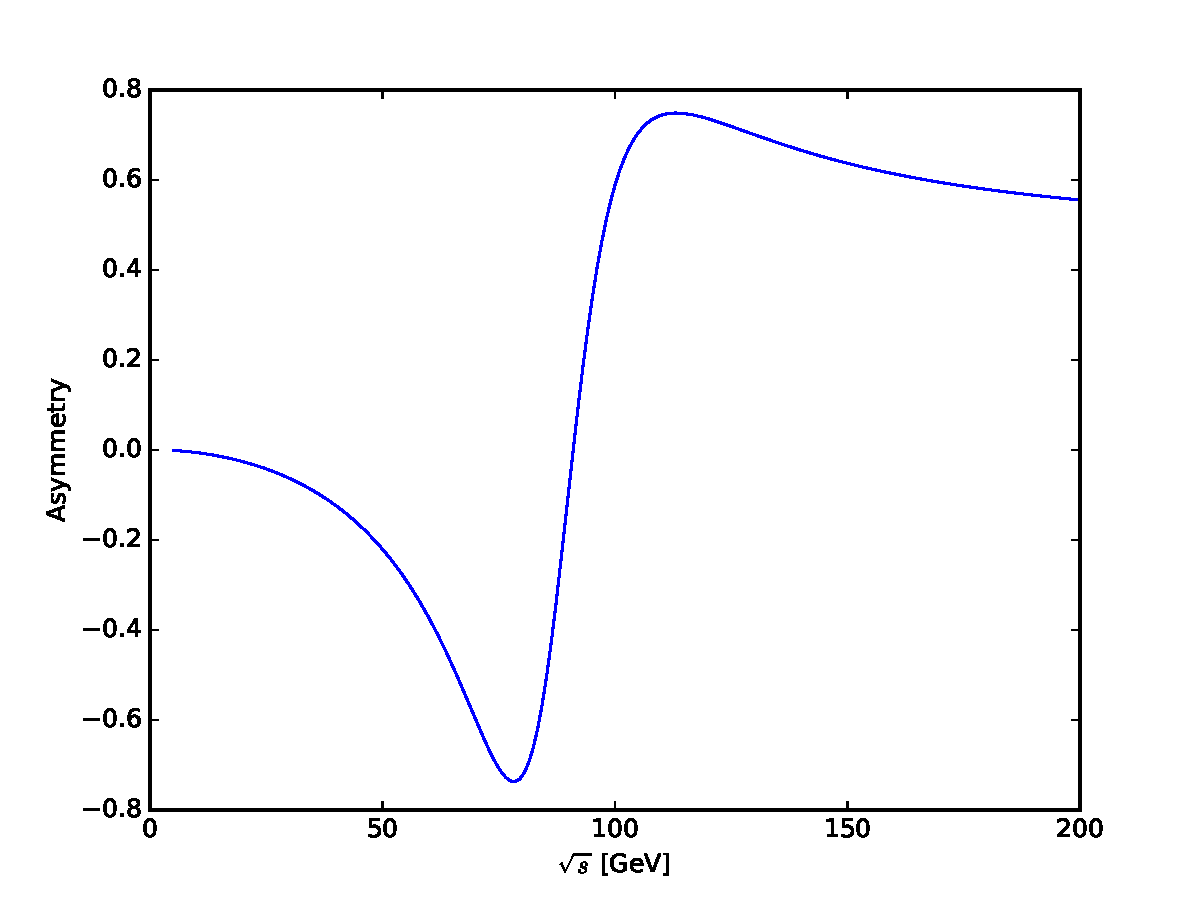
\includegraphics[width=\textwidth]{../tables/ZAsym.pdf}
    \caption{Forward backward asymmetry}
  \end{subfigure}
  ~
  \begin{subfigure}[b]{0.45\textwidth}
    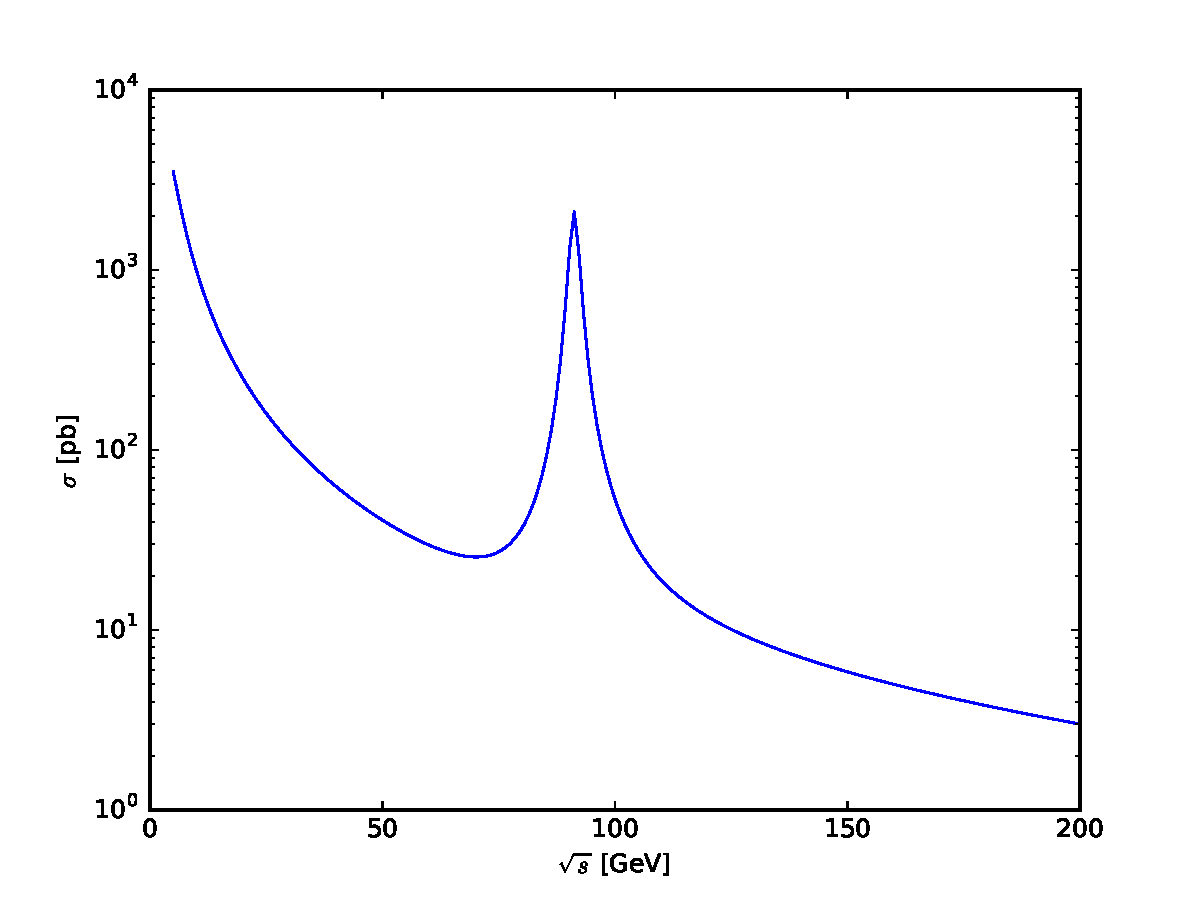
\includegraphics[width=\textwidth]{../tables/ZCross.pdf}
    \caption{Total cross section}
  \end{subfigure}
\end{figure}
\newpage
\section{Dilepton production beyond the SM}

\subsection{$Z'$}
Almost any grand unified theory perdicts the existence of a $Z'$. $Z'$ would be
involved in the same lepton production as $Z$ only it would need much more
energy due to its mass.
Finding the $Z'$ could give clues to how the forces relate to one another, or give
information about the characteristics of extra dimensions.

\subsection{Cross section and $A_{FB}$}
\begin{figure}[h!]
  \caption{$e^+e^-\rightarrow \gamma,Z,Z' \rightarrow \mu^+\mu^-$}
  \centering
  \begin{subfigure}[b]{0.45\textwidth}
    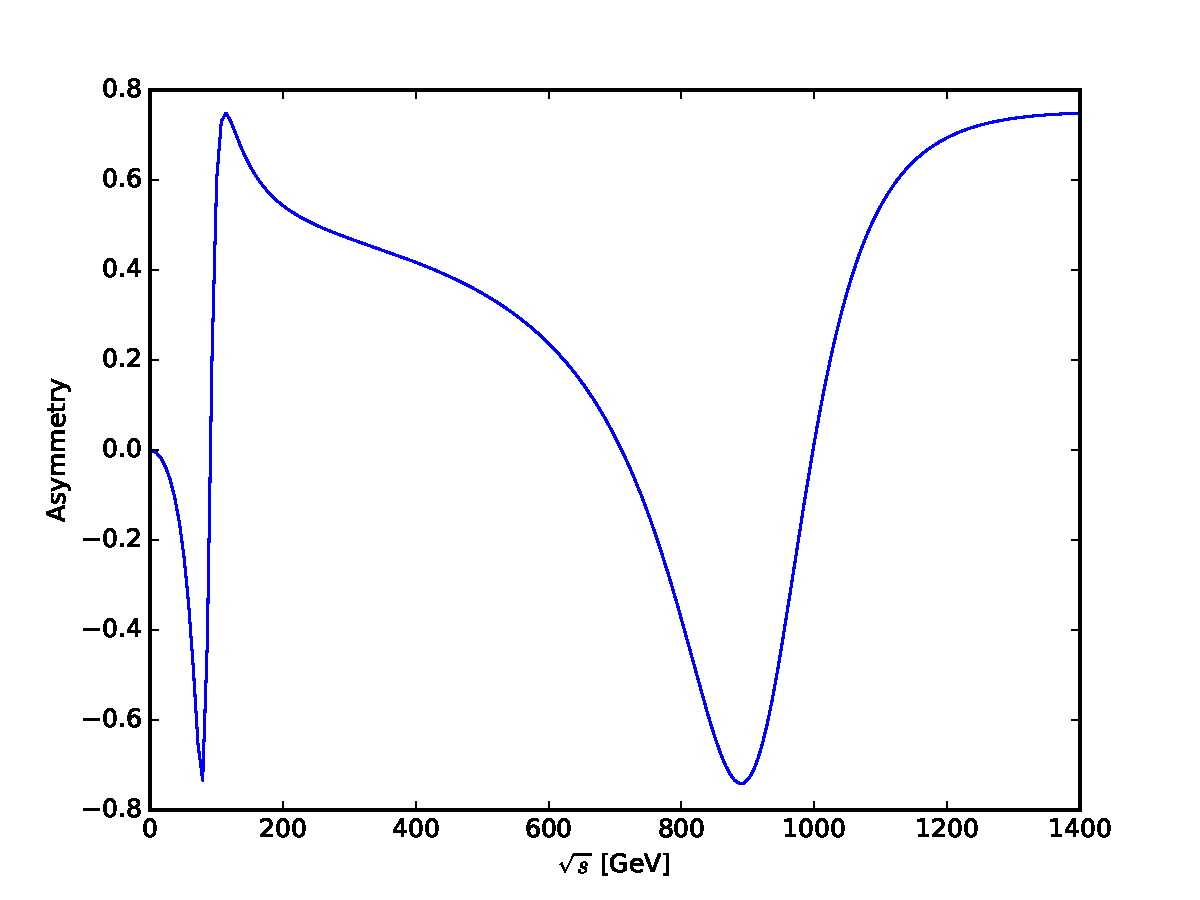
\includegraphics[width=\textwidth]{../tables/ZpAsym.pdf}
    \caption{Forward backward asymmetry with $Z'$ included}
  \end{subfigure}
  ~
  \begin{subfigure}[b]{0.45\textwidth}
    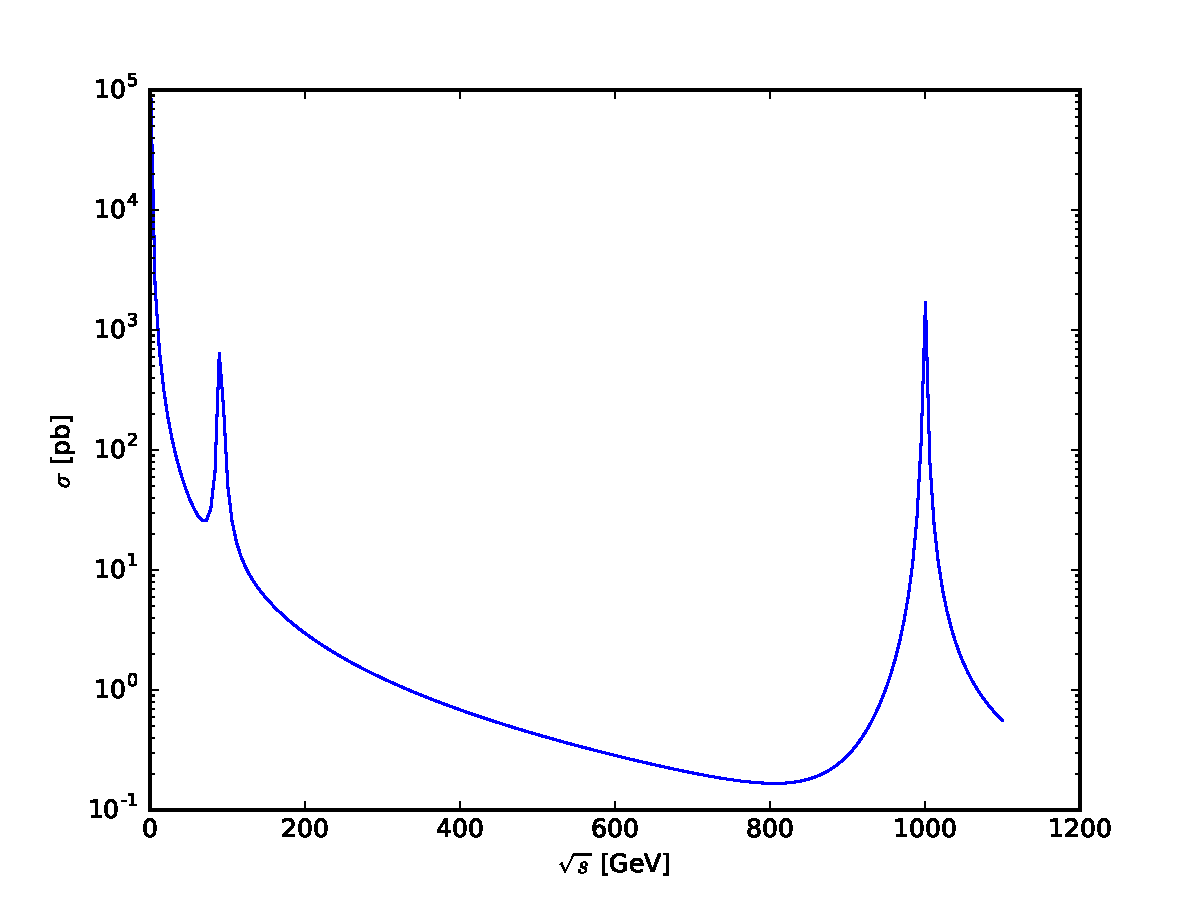
\includegraphics[width=\textwidth]{../tables/ZpCross.pdf}
    \caption{Total cross section with}
  \end{subfigure}
\end{figure}
%
In the cross section graph we see two large spikes around the $Z$ and $Z'$ masses
showing the favourability around these processes under these masses. We can see the
same behaviour in the $A_{FB}$ plot.

\subsection{$Z'$ and $W'$ production}
$Z'$ would be produced in hadron colliders due to the need for high energies.
The $Z'$ would be produced from an $q\bar{q}$ annihilation from where it would
decay into dilepton- or diquark pair. As for the $W'$ it would alse come from a $q\bar{q}$
annihilation and decay into lepton and neutrino, or top and bottom quark.
From an article from 2011\footnote{http://pdg.lbl.gov/2011/reviews/rpp2011-rev-wprime-searches.pdf}
the ATLAS Experiment had a cross section using the cross section from 
$pp \rightarrow W'X$ at about $1\,fb^{-1}$, times the branching ratio of 
$W'\rightarrow e\nu$ which gives a cross section of about $100\,fb$ for a $W'$ mass of $500\,GeV$. 
In the search for $W'$ we are looking for a high missing transverse mass, in where the transverse
mass is 
\[ m_T^2 = m^2 + p_x^2 + p_y^2\]
so it is the sum of the invariant mass and $p_T$.

\subsection{Slepton pair production}
There would be an energy difference in the signals

\end {document}



























